\section{Numerical Evaluation and Controlled Comparisons}\label{sec:experiments}

\subsection{Tasks, Evaluation Criteria, and Comparison Levels}
Single-integrator experiments use $\ds=1.000\ \mathrm m$, $U=0.50\ \mathrm{m/s}$, workspace $[-4,4]^2\ \mathrm m^2$, polynomial channel radius $R_c=10.0\ \mathrm m$, communication radius $2.50\ \mathrm m$, barrier decay rates $2.0\ \mathrm s^{-1}$, nominal control period $0.05\ \mathrm s$, and horizon $60\ \mathrm s$. Initial triangular-lattice spacing is $1.001\ \mathrm m$. Safe arrival requires maximum goal error at most $0.01\ \mathrm m$ for at least $1.0\ \mathrm s$ measured from timestamps, with all executed segments passing the same rational safety audit. Commands are integrated without position clipping. Any certificate-induced reduction in holding time is recorded as part of the controller.

We distinguish performance of a specified frozen policy, execution-time interventions holding its weights fixed, and comparisons between learning variants with matched training budgets and seeds. The analytical references use either $\bu_i^{\mathrm{nom}}=-\be_i$ or a constant tangential residual with $\omega_i=1,r_i=\psi_{ij}=0$, followed by the same NPA shield. These are explicitly defined references related to CBF projection and circulation\cite{ames2017cbf,goncalves2023circulation}, rather than reproductions of every component of those published methods.

GCBF+\cite{zhang2025gcbf} and DGPPO\cite{zhang2025dgppo} learn barrier functions that differ from static allocation. Replacing NPA by static allocation does not implement their algorithms. The projection-penalty variant also uses our policy and shield. Both are internal comparisons. Section~\ref{subsec:external} separately uses the official DGPPO update with an explicit adaptation to our dynamics and spectral constraint; no DGPPO performance is inferred from internal variants.

We separately record certification stops, solver failures, computational-budget exhaustion, zero-speed stalls, physical-horizon timeouts, and safe arrivals. Existing shield evaluations allow at most $3600$ controller calls; $100$ consecutive calls with total speed norm below $10^{-6}\ \mathrm{m/s}$ are classified as a stall. A certified prefix ending early is not counted as a completed safe horizon. Paired arrival times use common safe arrivals; we additionally report mean completion time with failures assigned $60\ \mathrm s$. Training replicates are reported separately; scenarios evaluated using one policy are not independent training replicates.

\subsection{Performance of the Specified Frozen Policy}
The original policy receives approximately $9.63\times10^5$ environment steps and one checkpoint is selected on validation tasks. Fig.~\ref{fig:train-curves} shows this training run. The development benchmark comprises $64$ tasks at $N=8$ and $32$ cross-scale tasks. The former contains $20$ local swaps and $12$ permutations at each of $f=\lr/\lambda_2(\bL(\bp_0))=0.60,0.90$. The latter contains $12,12,8$ tasks at $N=12,20,25$, respectively, with $f=0.60$. Initial states, goal assignments, and safety requirements are shared within each task.

\begin{figure*}[t]
\centering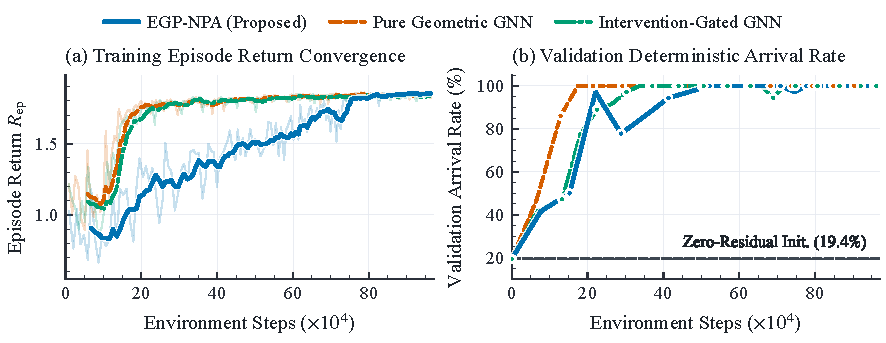
\includegraphics[width=\textwidth]{figures_en/fig2_training_curves.pdf}
\caption{Full-budget returns and validation success for the original policy and separately trained configurations. Each curve is one training run, rather than a mean or confidence interval across seeds.}\label{fig:train-curves}
\end{figure*}

\begin{table*}[t]
\centering\footnotesize
\caption{Specified Checkpoint and Analytical References on the $N=8$ Development Benchmark; Times Are Medians Among Safe Arrivals}\label{tab:e1}
\begin{tabularx}{\textwidth}{@{}Xcccccc@{}}\toprule
Controller & $f=.60$ Arrivals & Time/s & $f=.90$ Arrivals & Time/s & Step Cuts & Failed Audit Segments\\\midrule
EGP-NPA, $B=8$ & $32/32$ & $7.32$ & $32/32$ & $7.12$ & $0$ & $0$\\
Constant tangential residual + NPA & $21/32$ & $32.50$ & $18/32$ & $30.50$ & $0$ & $0$\\
Proportional attraction + NPA & $17/32$ & $36.35$ & $16/32$ & $31.80$ & $0$ & $0$\\
\bottomrule\end{tabularx}
\end{table*}

\begin{table*}[t]
\centering\footnotesize
\caption{Cross-Scale Performance of the Specified Checkpoint and Analytical References; Parentheses Give Median Safe-Arrival Time/s}\label{tab:e2}
\begin{tabularx}{\textwidth}{@{}Xccccr@{}}\toprule
Controller & $N=12$ & $N=20$ & $N=25$ & Total & Step Cuts\\\midrule
EGP-NPA, $B=8$ & $12/12\ (6.52)$ & $12/12\ (10.55)$ & $8/8\ (10.43)$ & $32/32$ & $0$\\
Constant tangential residual + NPA & $7/12\ (14.40)$ & $4/12\ (24.53)$ & $2/8\ (38.22)$ & $13/32$ & $14198$\\
Proportional attraction + NPA & $4/12\ (34.30)$ & $1/12\ (55.50)$ & $0/8\ (\text{---})$ & $5/32$ & $0$\\
\bottomrule\end{tabularx}
\end{table*}

Tables~\ref{tab:e1}--\ref{tab:e2} report $96/96$ safe arrivals for the specified checkpoint; it also achieves $48/48$ on an additional held-out set. These percentages describe that checkpoint on those tasks. It is not ranked against lower-budget learning runs as evidence of algorithm-level superiority. Training variability is examined separately below.

\subsection{Learning Variants With Matched Budgets and Seeds}\label{subsec:matched}
A $2\times2$ factorial design varies team/local critics and the projection penalty, with two training replicates per cell. All variants share the 17-dimensional node and 20-dimensional edge observations, two-layer equivariant actor, training distribution, reward, $B=2$ training shield, and validation selection rule. Corresponding replicates use matched initialization and scene random seeds. Each run receives a budget of $480000$ environment transitions, ending at a complete sampling batch; actual totals range from $481274$ to $487089$. All eight checkpoints are evaluated on the same $48$ held-out tasks with the completion envelope and $B=8$, giving $384$ retained runs and zero failed audit segments or step cuts.

The penalty is $\mathcal L_{\mathrm{proj}}=\lambda_{\mathrm{proj}}N^{-1}\sum_i\norm{\Pi_{\mathcal U_i}(\bu_i^{\mathrm{nom}})-\operatorname{sg}(\bu_i)}_2^2$, where $\operatorname{sg}$ denotes stop-gradient and $\lambda_{\mathrm{proj}}\in\{0,1\}$. Its nonzero weight is calibrated using gradient scales before training. The common validation rule selects different training stages: team-critic base checkpoints at approximately $216000/401000$ steps and penalized checkpoints at $71000/73000$ steps; local-critic counterparts at $360000/420000$ and $140000/129000$ steps. The comparison therefore concerns the complete training-and-selection procedure.

\begin{table*}[t]
\centering\footnotesize
\caption{Matched-Budget Internal Learning Variants. Semicolons Separate Training Replicates; Time Differences Are Penalty Minus Base on Common Safe Arrivals Within Each Seed}\label{tab:matched}
\begin{tabularx}{\textwidth}{@{}Xcccc@{}}\toprule
Critic & $\lambda_{\mathrm{proj}}$ & $N=8$ Safe Arrivals & Cross-Scale Safe Arrivals & Median Paired Difference/s\\\midrule
Team & 0 & $32/32\ ;\ 32/32$ & $12/16\ ;\ 14/16$ & --- \\
Team & 1 & $32/32\ ;\ 32/32$ & $9/16\ ;\ 11/16$ & $+0.00\ ;\ +1.60$ \\
Local & 0 & $32/32\ ;\ 32/32$ & $4/16\ ;\ 9/16$ & --- \\
Local & 1 & $31/32\ ;\ 32/32$ & $8/16\ ;\ 14/16$ & $+4.35\ ;\ +1.60$ \\
\bottomrule\end{tabularx}
\end{table*}

Table~\ref{tab:matched} exhibits a critic-dependent interaction. With team critics, the penalty loses three cross-scale arrivals in each replicate. With local critics, cross-scale arrivals increase from $4$ to $8$ and from $9$ to $14$. Median paired time differences are $0.00/1.60\ \mathrm s$ for team critics and $4.35/1.60\ \mathrm s$ for local critics. Assigning $60\ \mathrm s$ to cross-scale failures changes mean completion times from $28.23/20.49$ to $34.10/29.34\ \mathrm s$ for team critics, but improves them from $50.42/35.11$ to $39.32/22.88\ \mathrm s$ for local critics. Intervention reduction and task completion must consequently be evaluated separately. Two training replicates support a descriptive comparison, not an algorithm-level significance claim.

\begin{figure*}[t]
\centering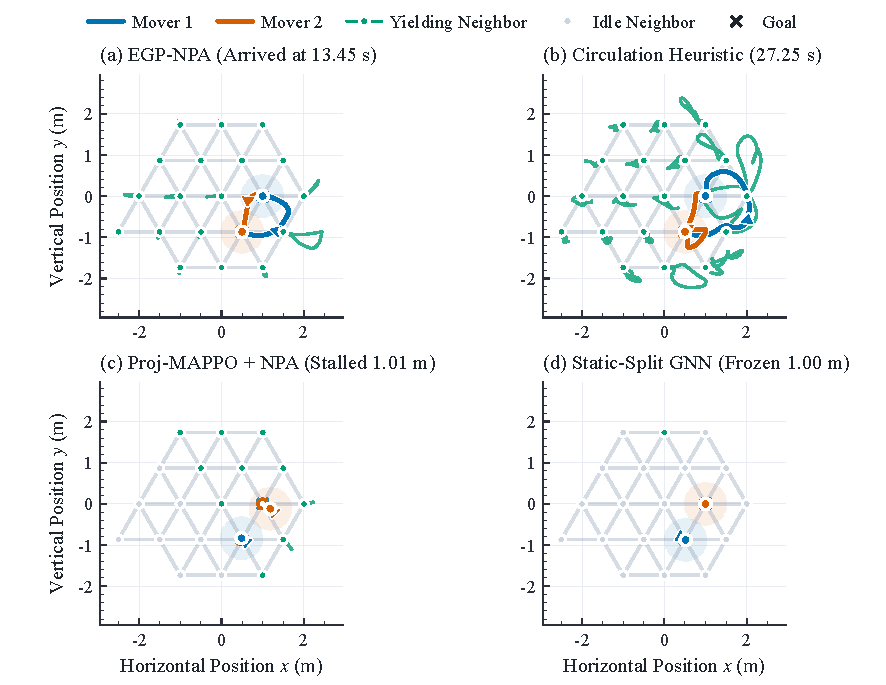
\includegraphics[width=\textwidth]{figures_en/fig3_swap_trajectory.pdf}
\caption{Matched-budget team-critic trajectories on one held-out $N=20$ swap. (a)--(b) Base and penalized policies from training replicate 1; (c)--(d) the corresponding pair from replicate 2. Initial states, goals, safety parameters, and axis limits are shared.}\label{fig:swap-traj}
\end{figure*}
\begin{figure*}[t]
\centering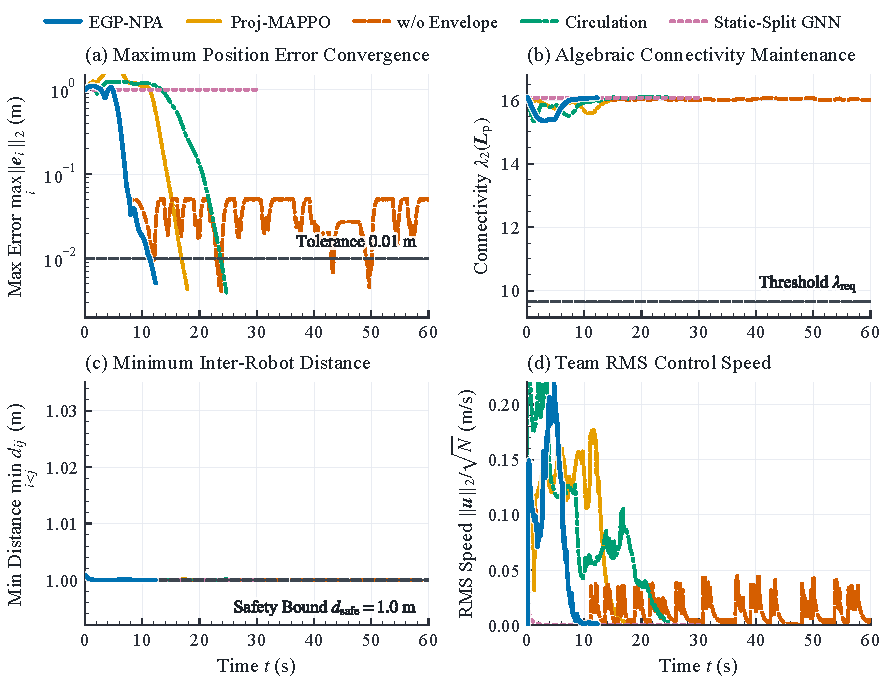
\includegraphics[width=\textwidth]{figures_en/fig4_time_evolution.pdf}
\caption{Time responses for the same task and four matched policies in Fig.~\ref{fig:swap-traj}: maximum goal error, algebraic connectivity, minimum distance, and RMS speed. Curves use stored executed trajectories without extending terminated runs.}\label{fig:time-evol}
\end{figure*}

\subsection{Fixed-Weight Ablations and Failure Categories}\label{subsec:ablation}
Keeping the original policy weights fixed while replacing $B=8$ with $B=0$ yields $11/64$ safe arrivals at $N=8$ and $1/32$ across larger teams. This is an execution-time shield replacement for a policy trained with dynamic allocation, not a separately trained competing algorithm. Table~\ref{tab:static-status} retains all termination categories; $51$ certification or computational-budget stops are distinguished from zero-speed stalls.

\begin{table}[t]
\centering\footnotesize
\caption{All Static-Allocation Ablation Outcomes}\label{tab:static-status}
\begin{tabular}{@{}lrr@{}}\toprule
Termination & $N=8$ & Cross-Scale\\\midrule
Safe arrival & 11 & 1\\
Certification stop & 30 & 7\\
Controller-call budget & 7 & 7\\
Zero-speed stall & 12 & 13\\
Physical-horizon timeout & 4 & 4\\\bottomrule
\end{tabular}
\end{table}

For one $N=20$ task over $[0.05,1.00]\ \mathrm s$, identical nominal inputs yield lateral executed speeds $0.2003/0.0004\ \mathrm{m/s}$ under dynamic/static allocation and outward neighbor speeds $0.0915/0.0013\ \mathrm{m/s}$. This local intervention is consistent with the two-node yielding mechanism of Proposition~\ref{prop:unfreeze}; failure categories for complete multi-contact tasks remain those in Table~\ref{tab:static-status}.

\begin{table*}[t]
\centering\footnotesize
\caption{Internal Interventions, Distinguishing Separate Training Runs From Fixed-Weight Execution Changes}\label{tab:decomp}
\begin{tabularx}{\textwidth}{@{}Xlc@{}}\toprule
Configuration & Comparison Type & Safe Arrivals\\\midrule
Complete policy and envelope & Reference checkpoint & $32/32$\\
Remove completion envelope & Fixed-weight execution change & $25/32$\\
Geometric-only observations & Separately trained checkpoint & $22/32$\\
Intervention-based gate training & Separately trained checkpoint & $15/32$\\\midrule
Original / envelope-only / replaced gate & Fixed weights, 16-task subset & $16/16$ each\\
Zero collision-price features & Fixed weights, 16-task subset & $16/16$\\
Zero collision-ledger features & Fixed weights, 16-task subset & $16/16$\\
Zero all algebraic features & Fixed weights, 16-task subset & $15/16$\\\bottomrule
\end{tabularx}
\end{table*}

Terminal hovering after envelope removal demonstrates the component's practical role for this policy. Differences between separate checkpoints also include training variation; execution-time feature removal probes sensitivity of a trained policy rather than the value of those features after retraining. Reflection symmetrization at inference reduces arrivals from $48$ to $30$ on the held-out set, describing this deterministic policy intervention and its connection to the exactly symmetric head-on analysis.

\begin{figure*}[t]
\centering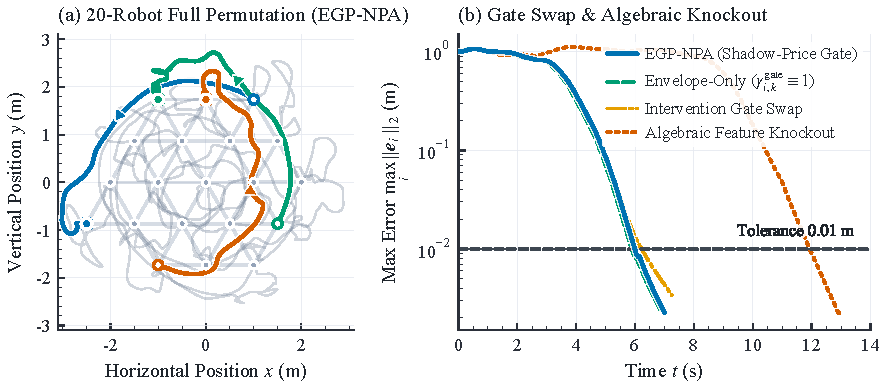
\includegraphics[width=\textwidth]{figures_en/fig5_perm_and_gate.pdf}
\caption{Permutation-task trajectories and fixed-weight gate/feature interventions. Training-configuration comparisons and execution-time interventions are evaluated separately.}\label{fig:perm-gate}
\end{figure*}

The custom unshielded Lagrangian PPO is retained as an exploratory negative result. It uses 12/13-dimensional geometric inputs and at most $264000$ training transitions. Its last logged average cost is approximately $0.929$, exceeding its training limit $0.02$. Re-evaluating the same checkpoint with an elapsed $1.0\ \mathrm s$ holding rule and without workspace position clipping still produces collisions in all $96$ development tasks. This training configuration has not met the task constraints; its failure is not used to infer the general capability of primal--dual learning or the necessity of our particular shield.

\subsection{Separate Boundary Evaluation With Second-Order Physics}\label{subsec:mujoco}
The \texttt{MuJoCo} evaluation uses robot mass $6.0\ \mathrm{kg}$, body radius $0.45\ \mathrm m$, velocity-loop time constant $45\ \mathrm{ms}$, thrust limit $22.0\ \mathrm N$, physics step $5\ \mathrm{ms}$, and control period $50\ \mathrm{ms}$. Each control step has six spectral-consensus rounds and four NPA rounds. Observation delay is $10\ \mathrm{ms}$, communication delay is $5$--$15\ \mathrm{ms}$, and packet loss is $2\%$. These runs are reported separately from the single-integrator comparisons.

\begin{table*}[t]
\centering\footnotesize
\caption{Physical Arrivals and Safety Boundaries. Arrivals Do Not Require Violation-Free Motion; Distance Is the Minimum and Violation Steps Are Averaged Over Four Tasks}\label{tab:mujoco}
\begin{tabularx}{\textwidth}{@{}lcXcrr@{}}\toprule
Regime & $N$ & Configuration & Arrivals & Min Distance/m & Viol. Steps\\\midrule
A & 8 & Attraction + physical interface & $0/4$ & .9817 & 610.2\\
A & 8 & Learned policy + static allocation & $1/4$ & .9798 & 442.2\\
A & 8 & Learned policy + uncompensated filter & $0/4$ & .9792 & 4231.0\\
A & 8 & Learned policy + online spectrum + physical interface & $3/4$ & .8990 & 1683.5\\
A & 12 & Attraction + physical interface & $0/4$ & .9952 & 1679.2\\
A & 12 & Learned policy + static allocation & $0/4$ & .9976 & 850.8\\
A & 12 & Learned policy + uncompensated filter & $0/4$ & .9937 & 4190.2\\
A & 12 & Learned policy + online spectrum + physical interface & $1/4$ & .8988 & 2777.0\\\midrule
B & 8 & Attraction + physical interface & $0/4$ & 1.0240 & 0\\
B & 8 & Learned policy + static allocation & $0/4$ & 1.0260 & 0\\
B & 8 & Learned policy + uncompensated filter & $0/4$ & .8987 & 4722.0\\
B & 8 & Learned policy + online spectrum + physical interface & $0/4$ & .9910 & 1133.2\\
B & 12 & Attraction + physical interface & $0/4$ & 1.0256 & 0\\
B & 12 & Learned policy + static allocation & $0/4$ & 1.0255 & 0\\
B & 12 & Learned policy + uncompensated filter & $0/4$ & .9809 & 4783.2\\
B & 12 & Learned policy + online spectrum + physical interface & $0/4$ & 1.0096 & 0\\\bottomrule
\end{tabularx}
\end{table*}

Regime A uses spacing $1.018\ \mathrm m$. Regime B uses spacing $1.045\ \mathrm m$, distance tightening $0.028\ \mathrm m$, and command-increment limit $0.22\ \mathrm{m/s}$. Table~\ref{tab:mujoco} retains negative full-stack outcomes: regime A has arrivals with distance violations; regime B has no arrivals in eight tasks, with seven collision-violation-free runs and one $N=8$ task reaching $0.9910\ \mathrm m$. All $64$ physical runs record zero connectivity violations. Accurate spectrum tracking does not imply simultaneous collision avoidance, and the single-integrator safety statement does not directly cover actuator lag and post-filter command limiting.

\begin{figure*}[t]
\centering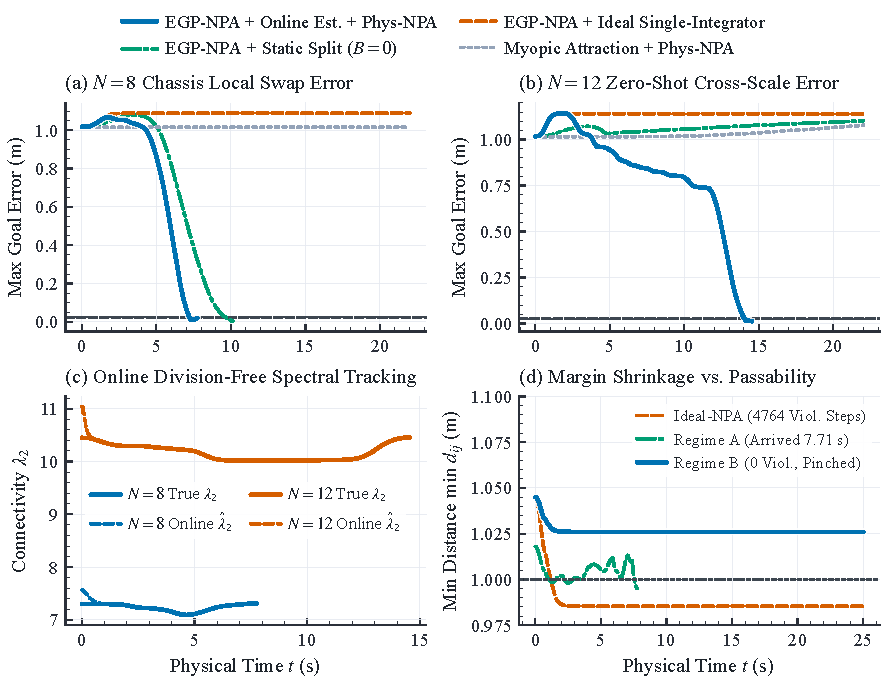
\includegraphics[width=\textwidth]{figures_en/fig6_mujoco_verification.pdf}
\caption{Second-order closed-loop goal error, online spectral estimation, and distance responses. Violations and nonarrivals are retained for both compensation regimes.}\label{fig:mujoco}
\end{figure*}

\begin{theorem}[Initial Feasibility and a Specified Crossing Section]\label{thm:passability-tradeoff}
Let $D=\ds+\Delta d_{\mathrm{phys}}$. Initial distance constraints are strictly feasible exactly when $D<S$, where $S$ is the minimum initial spacing. Consider only a symmetric four-node crossing section whose perpendicular diagonals share a midpoint, with moving-node diagonal fixed at $D$ and the other diagonal equal to $b$. All adjacent distances are at least $D$ exactly when $b\ge\sqrt3D$.
\end{theorem}
\begin{proof}
The first claim follows from the definition of minimum initial distance. Each adjacent side in the specified section has length $\sqrt{D^2+b^2}/2$, so the required inequality is equivalent to $b^2\ge3D^2$. The diagonals $D$ and $b\ge\sqrt3D$ also satisfy the distance requirement.
\end{proof}
This theorem concerns the specified section. General rearrangements permit asymmetric detours and motion of outer robots; path connectedness of the full configuration space requires a separate analysis.
